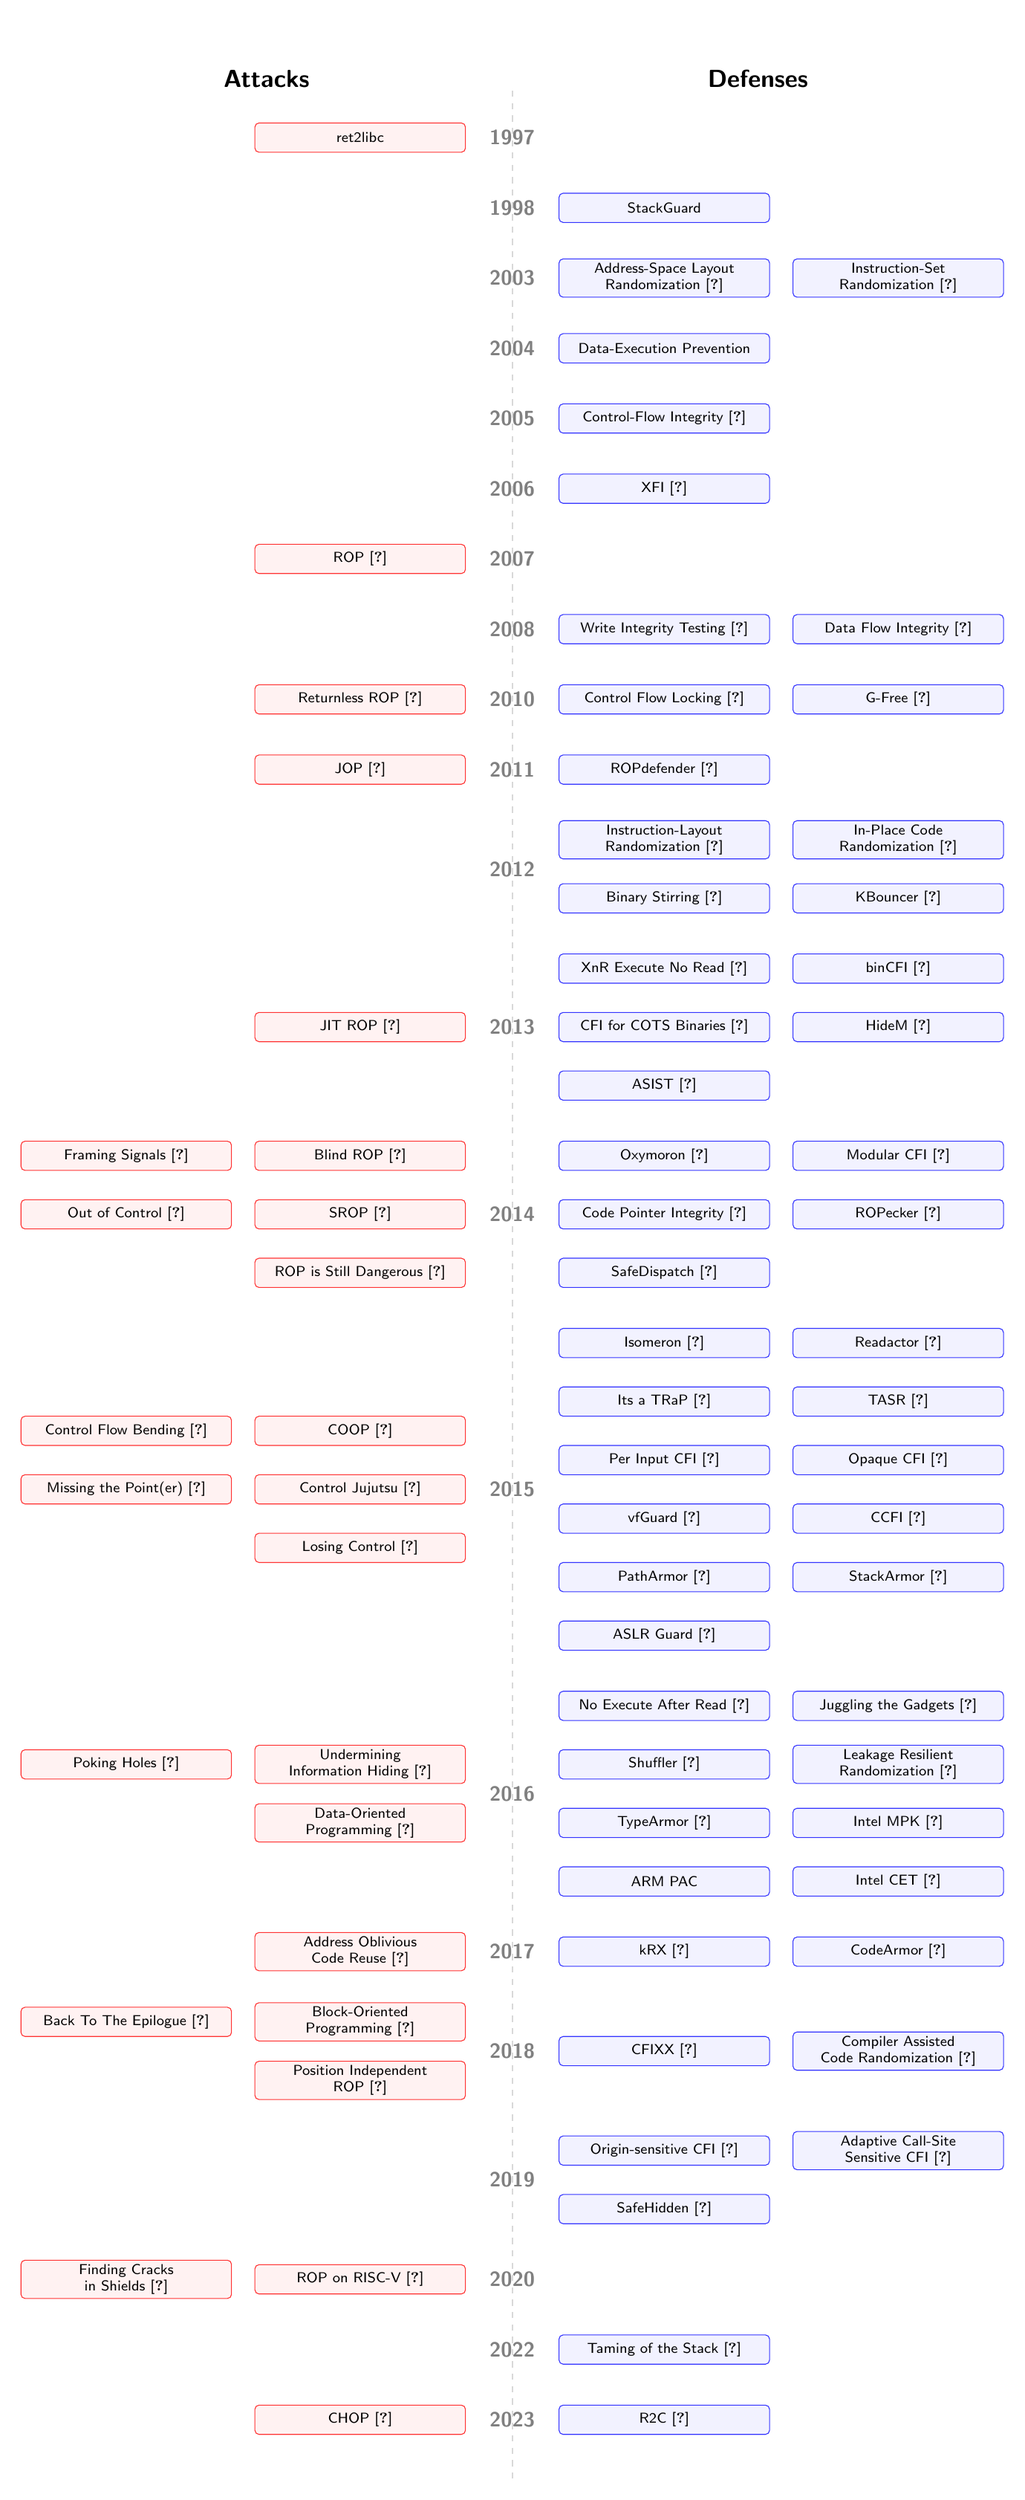
\begin{tikzpicture}[year node/.style={font=\bfseries\sffamily\color{gray}, align=center, inner sep=2pt},attack node/.style={draw=red!80, fill=red!5, rounded corners=2pt, font=\scriptsize\sffamily, align=center, minimum width=3.60cm, minimum height=0.5cm, inner sep=2pt, text width=3.40cm, execute at begin node=\setlength{\emergencystretch}{0pt}\tolerance 200\hyphenpenalty 10000\exhyphenpenalty 10000},defense node/.style={draw=blue!80, fill=blue!5, rounded corners=2pt, font=\scriptsize\sffamily, align=center, minimum width=3.60cm, minimum height=0.5cm, inner sep=2pt, text width=3.40cm, execute at begin node=\setlength{\emergencystretch}{0pt}\tolerance 200\hyphenpenalty 10000\exhyphenpenalty 10000},spine/.style={thick, gray!30, dashed}]%
\node[font=\large\bfseries\sffamily] at (-4.2,1.0) {Attacks};%
\node[font=\large\bfseries\sffamily] at (4.2,1.0) {Defenses};%
  % Year 1997%
\node[year node] at (0.0,0.0) {1997};%
\node[attack node] at (-2.6,0.0) {ret2libc};%
  % Year 1998%
\node[year node] at (0.0,-1.2) {1998};%
\node[defense node] at (2.6,-1.2) {StackGuard};%
  % Year 2003%
\node[year node] at (0.0,-2.4) {2003};%
\node[defense node] at (2.6,-2.4) {Address{-}Space Layout\\ Randomization \allowbreak\cite{PaXTeam2003}};%
\node[defense node] at (6.6,-2.4) {Instruction{-}Set\\ Randomization \allowbreak\cite{boyd2010}};%
  % Year 2004%
\node[year node] at (0.0,-3.6) {2004};%
\node[defense node] at (2.6,-3.6) {Data{-}Execution Prevention};%
  % Year 2005%
\node[year node] at (0.0,-4.8) {2005};%
\node[defense node] at (2.6,-4.8) {Control{-}Flow Integrity \allowbreak\cite{Abadi2005}};%
  % Year 2006%
\node[year node] at (0.0,-6.0) {2006};%
\node[defense node] at (2.6,-6.0) {XFI \allowbreak\cite{Erlingsson2006}};%
  % Year 2007%
\node[year node] at (0.0,-7.2) {2007};%
\node[attack node] at (-2.6,-7.2) {ROP \allowbreak\cite{Shacham2007}};%
  % Year 2008%
\node[year node] at (0.0,-8.4) {2008};%
\node[defense node] at (2.6,-8.4) {Write Integrity Testing \allowbreak\cite{Akritidis2008}};%
\node[defense node] at (6.6,-8.4) {Data Flow Integrity \allowbreak\cite{castro2006}};%
  % Year 2010%
\node[year node] at (0.0,-9.6) {2010};%
\node[attack node] at (-2.6,-9.6) {Returnless ROP \allowbreak\cite{checkoway2010}};%
\node[defense node] at (2.6,-9.6) {Control Flow Locking \allowbreak\cite{Bletsch2011b}};%
\node[defense node] at (6.6,-9.6) {G{-}Free \allowbreak\cite{Onarlioglu2010}};%
  % Year 2011%
\node[year node] at (0.0,-10.8) {2011};%
\node[attack node] at (-2.6,-10.8) {JOP \allowbreak\cite{Bletsch2011a}};%
\node[defense node] at (2.6,-10.8) {ROPdefender \allowbreak\cite{davi2011}};%
  % Year 2012%
\node[year node] at (0.0,-12.5) {2012};%
\node[defense node] at (2.6,-12.0) {Instruction{-}Layout\\ Randomization \allowbreak\cite{Hiser2012}};%
\node[defense node] at (6.6,-12.0) {In{-}Place Code\\ Randomization \allowbreak\cite{Pappas2012a}};%
\node[defense node] at (2.6,-13.0) {Binary Stirring \allowbreak\cite{Wartell2012}};%
\node[defense node] at (6.6,-13.0) {KBouncer \allowbreak\cite{Pappas2013b}};%
  % Year 2013%
\node[year node] at (0.0,-15.2) {2013};%
\node[attack node] at (-2.6,-15.2) {JIT ROP \allowbreak\cite{Snow2013}};%
\node[defense node] at (2.6,-14.2) {XnR Execute No Read \allowbreak\cite{Backes2013}};%
\node[defense node] at (6.6,-14.2) {binCFI \allowbreak\cite{zhang2013}};%
\node[defense node] at (2.6,-15.2) {CFI for COTS Binaries \allowbreak\cite{zhang2013}};%
\node[defense node] at (6.6,-15.2) {HideM \allowbreak\cite{Goktas2016b}};%
\node[defense node] at (2.6,-16.2) {ASIST \allowbreak\cite{papadogiannakis2013}};%
  % Year 2014%
\node[year node] at (0.0,-18.4) {2014};%
\node[attack node] at (-2.6,-17.4) {Blind ROP \allowbreak\cite{Bittau2014a}};%
\node[attack node] at (-6.6,-17.4) {Framing Signals \allowbreak\cite{Bittau2014a}};%
\node[attack node] at (-2.6,-18.4) {SROP \allowbreak\cite{bosman2014}};%
\node[attack node] at (-6.6,-18.4) {Out of Control \allowbreak\cite{Goktas2016b}};%
\node[attack node] at (-2.6,-19.4) {ROP is Still Dangerous \allowbreak\cite{carlini2014}};%
\node[defense node] at (2.6,-17.4) {Oxymoron \allowbreak\cite{Backes2014f}};%
\node[defense node] at (6.6,-17.4) {Modular CFI \allowbreak\cite{niu2014}};%
\node[defense node] at (2.6,-18.4) {Code Pointer Integrity \allowbreak\cite{Kuznetsov2014}};%
\node[defense node] at (6.6,-18.4) {ROPecker \allowbreak\cite{Cheng2014}};%
\node[defense node] at (2.6,-19.4) {SafeDispatch \allowbreak\cite{jang2014}};%
  % Year 2015%
\node[year node] at (0.0,-23.1) {2015};%
\node[attack node] at (-2.6,-22.1) {COOP \allowbreak\cite{Schuster2015a}};%
\node[attack node] at (-6.6,-22.1) {Control Flow Bending \allowbreak\cite{Carlini2015}};%
\node[attack node] at (-2.6,-23.1) {Control Jujutsu \allowbreak\cite{Evans2015a}};%
\node[attack node] at (-6.6,-23.1) {Missing the Point(er) \allowbreak\cite{Evans2015}};%
\node[attack node] at (-2.6,-24.1) {Losing Control \allowbreak\cite{conti2015}};%
\node[defense node] at (2.6,-20.6) {Isomeron \allowbreak\cite{Davi2015}};%
\node[defense node] at (6.6,-20.6) {Readactor \allowbreak\cite{Crane2015}};%
\node[defense node] at (2.6,-21.6) {Its a TRaP \allowbreak\cite{Crane2015b}};%
\node[defense node] at (6.6,-21.6) {TASR \allowbreak\cite{bigelow2015}};%
\node[defense node] at (2.6,-22.6) {Per Input CFI \allowbreak\cite{Niu2015}};%
\node[defense node] at (6.6,-22.6) {Opaque CFI \allowbreak\cite{Mohan2015}};%
\node[defense node] at (2.6,-23.6) {vfGuard \allowbreak\cite{Prakash2015}};%
\node[defense node] at (6.6,-23.6) {CCFI \allowbreak\cite{Mashtizadeh2015}};%
\node[defense node] at (2.6,-24.6) {PathArmor \allowbreak\cite{Goktas2016b}};%
\node[defense node] at (6.6,-24.6) {StackArmor \allowbreak\cite{Chen2015c}};%
\node[defense node] at (2.6,-25.6) {ASLR Guard \allowbreak\cite{Lu2015}};%
  % Year 2016%
\node[year node] at (0.0,-28.3) {2016};%
\node[attack node] at (-2.6,-27.8) {Undermining\\ Information Hiding \allowbreak\cite{Goktas2016}};%
\node[attack node] at (-6.6,-27.8) {Poking Holes \allowbreak\cite{Oikonomopoulos2016a}};%
\node[attack node] at (-2.6,-28.8) {Data{-}Oriented\\ Programming \allowbreak\cite{Hu2016}};%
\node[defense node] at (2.6,-26.8) {No Execute After Read \allowbreak\cite{Werner2016}};%
\node[defense node] at (6.6,-26.8) {Juggling the Gadgets \allowbreak\cite{koo2016}};%
\node[defense node] at (2.6,-27.8) {Shuffler \allowbreak\cite{WilliamsKing2016}};%
\node[defense node] at (6.6,-27.8) {Leakage Resilient\\ Randomization \allowbreak\cite{Braden2016}};%
\node[defense node] at (2.6,-28.8) {TypeArmor \allowbreak\cite{VanderVeen2015b}};%
\node[defense node] at (6.6,-28.8) {Intel MPK \allowbreak\cite{Wahbe1993}};%
\node[defense node] at (2.6,-29.8) {ARM PAC};%
\node[defense node] at (6.6,-29.8) {Intel CET \allowbreak\cite{IntelCET}};%
  % Year 2017%
\node[year node] at (0.0,-31.0) {2017};%
\node[attack node] at (-2.6,-31.0) {Address Oblivious\\ Code Reuse \allowbreak\cite{Rudd2017}};%
\node[defense node] at (2.6,-31.0) {kRX \allowbreak\cite{Pomonis2019}};%
\node[defense node] at (6.6,-31.0) {CodeArmor \allowbreak\cite{Chen2017a}};%
  % Year 2018%
\node[year node] at (0.0,-32.7) {2018};%
\node[attack node] at (-2.6,-32.2) {Block{-}Oriented\\ Programming \allowbreak\cite{Ispoglou2018}};%
\node[attack node] at (-6.6,-32.2) {Back To The Epilogue \allowbreak\cite{biondo2018}};%
\node[attack node] at (-2.6,-33.2) {Position Independent\\ ROP \allowbreak\cite{Goktas2018}};%
\node[defense node] at (2.6,-32.7) {CFIXX \allowbreak\cite{Burow2018CFIXX}};%
\node[defense node] at (6.6,-32.7) {Compiler Assisted\\ Code Randomization \allowbreak\cite{Koo2018}};%
  % Year 2019%
\node[year node] at (0.0,-34.9) {2019};%
\node[defense node] at (2.6,-34.4) {Origin{-}sensitive CFI \allowbreak\cite{khandaker2019}};%
\node[defense node] at (6.6,-34.4) {Adaptive Call{-}Site\\ Sensitive CFI \allowbreak\cite{khandaker2019a}};%
\node[defense node] at (2.6,-35.4) {SafeHidden \allowbreak\cite{wang2019a}};%
  % Year 2020%
\node[year node] at (0.0,-36.6) {2020};%
\node[attack node] at (-2.6,-36.6) {ROP on RISC{-}V \allowbreak\cite{jaloyan2020}};%
\node[attack node] at (-6.6,-36.6) {Finding Cracks\\ in Shields \allowbreak\cite{li2020}};%
  % Year 2022%
\node[year node] at (0.0,-37.8) {2022};%
\node[defense node] at (2.6,-37.8) {Taming of the Stack \allowbreak\cite{huang2022a}};%
  % Year 2023%
\node[year node] at (0.0,-39.0) {2023};%
\node[attack node] at (-2.6,-39.0) {CHOP \allowbreak\cite{duta2023}};%
\node[defense node] at (2.6,-39.0) {R2C \allowbreak\cite{berlakovich2023}};%
\path[spine,draw] (0.0,0.8) -- (0.0,-40.0);%
\path[use as bounding box] (-8.40,-40.00) rectangle (8.40,2.00);%
\end{tikzpicture}